\exo{Type Brevet}{Brevet1} :On considère le programme de calcul suivant :

\begin{minipage}{0.4\textwidth}
    \begin{itemize}
        \item Choisir un nombre
        \item Le mettre au carré
        \item Multiplier par 5
        \item Ajouter 4
        \item Multiplier par 2
        \item Enlever 8
    \end{itemize}
\end{minipage}
\hfil
\begin{minipage}{0.55\textwidth}
    \begin{enumerate}
    \item Montrer que si 3 est le nombre de départ, le programme donne un résultat égal à 90.
    \item Un élève choisit 2 comme nombre de départ et un autre élève choisit $-2$. \\
    Montrer qu'ils doivent obtenir le même résultat.
    \item Si on nomme $x$ le nombre de départ, montrer que le résultat du programme peut s'écrire $10x^2$.
    \end{enumerate}
\end{minipage}


Light cherche le ou les nombre(s) qu'il doit choisir pour obtenir 30 comme résultat. Pour cela, il représente graphiquement la fonction $f$ associée au programme de calcul définie par : $f(x)=10x^2$.

\begin{center}
        \newcommand{\xmin}{-22}
        \newcommand{\xmax}{22}
        \newcommand{\ymin}{-5}
        \newcommand{\ymax}{45}
        \newcommand{\fnct}{f}
                        
                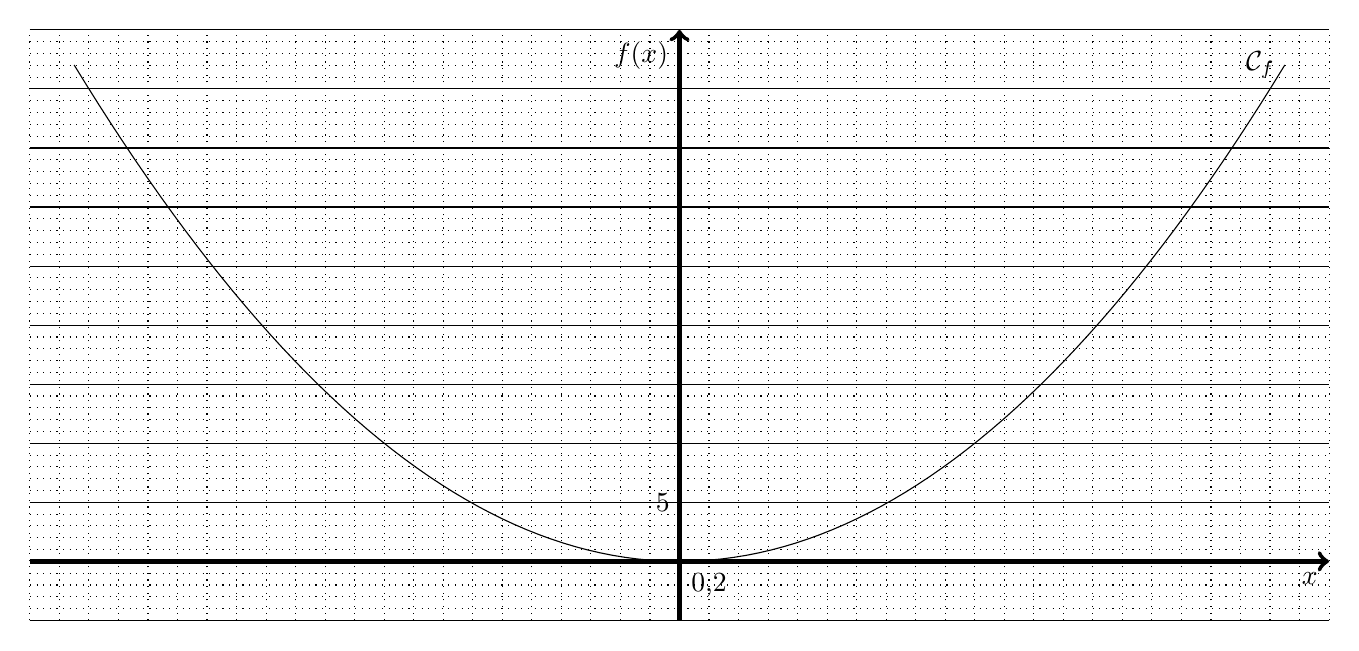
\begin{tikzpicture}[yscale=0.15,xscale=0.375]
                    \draw [dotted] (\xmin,\ymin) grid (\xmax,\ymax);
                    \draw [ultra thick,->] (0,\ymin)-- (0,\ymax) node[below left] {$\fnct(x)$};
                    \draw [ultra thick,->] (\xmin,0)-- (\xmax,0) node[below left] {$x$};
                    \draw[domain=\xmin +1.5: \xmax-1.5,samples=100]  plot (\x,\x*\x/10) node [left] {$\mathcal{C}_f$};
                    \draw (1,0.2)--(1,-0.2) node[below] {0,2};
                    \foreach \y in {-1,...,9}
                    {
                        \draw (\xmin,5*\y)--(\xmax,5*\y);
                    }
                    \node [left] at (0,5) {5};
                    
                \end{tikzpicture}
\end{center}

\begin{enumerate}[start=4]
    \item À l'aide du graphique, déterminer une valeur approchée des antécédents de 30 par la fonction $f$.

    \item Déterminer la valeur exacte du nombre positif cherché par l'élève.

\end{enumerate}
